\providecommand\ExamFontPath{../../../字体/}
\documentclass[fontset=exam]{exam-zh}
\usepackage{longtable,booktabs,array,calc,multirow,fvextra}
\usepackage[normalem]{ulem}
\providecommand{\hl}[1]{#1}
\providecommand{\ul}[1]{\uline{#1}}
\DefineVerbatimEnvironment{verbatim}{Verbatim}{breaklines=true,fontsize=\small}
\providecommand{\tightlist}{\setlength{\itemsep}{0pt}\setlength{\parskip}{0pt}}
\newcommand{\pandocbounded}[1]{#1}
\setlength{\emergencystretch}{3em}
\setlength{\tabcolsep}{2pt}
\examsetup{page/size=a4paper}
\title{期末考试}
\subject[4em]{离散数学}
\begin{document}
\maketitle
\fancyfoot[C]{第 \thepage 页（共 \pageref*{LastPage} 页）}
\begin{enumerate}
\item
  选择题.(每小题 2 分，总计 30)
\end{enumerate}

\begin{enumerate}
\def\labelenumi{\arabic{enumi}.}
\item
  给定语句如下：
\end{enumerate}

\begin{quote}
（1）15 是素数（质数）
\end{quote}

（2）10 能被 2 整除，3 是偶数。

（3）你下午有会吗？若无会，请到我这儿来！

（4）2x+3\textgreater0.

（5）只有 4 是偶数，3 才能被 2 整除。

(6)明年 5 月 1 日是晴天。

以上 6 个语句中，是简单命题的为（A）,是复合命题的为（B）,是真命题的为（C）,是假命题的是（D）,真值待定的命题是（E）

A: ①(1)(3)(4)(6) ②(1)(4)(6) ③(1)（6） B: ①(2)(4) ②(2)(4)(6) ③(2)(5)

C: ①(1)(2)(5)(6) ②无真命题 ③（5） D: ①(1)(2) ②无假命题 ③(1)(2)(4)(5)

E: ①(4)(6) ②（6） ③ 无真值待定的命题

\begin{enumerate}
\def\labelenumi{\arabic{enumi}.}
\setcounter{enumi}{1}
\item
  将下列语句符号化：
\end{enumerate}

（1）4 是偶数或是奇数。（A）设 p：4 是偶数，q：4 是奇数

（2）只有王荣努力学习，她才能取得好成绩。（B）设 p：王荣努力学习，q：王荣取得好成绩

（3）每列火车都比某些汽车快。（C）设 F(x):x 是火车，G(y):y 是汽车，H(x,y):x 比 y 快。

A: ① p\(\lor\)q ② p\(\land\)q ③ p\(\to\)q B: ① p\(\to\)q ② q\(\to\)p ③ p\(\land\)q

C: ①\(\forall\)\emph{x} \(\exists\)\emph{y} ((F(x) \(\land\)G(y)) \(\to\) (H(x,y))②\(\forall\)\emph{x} (F(x) \(\to\)\(\exists\)\emph{y}(G(y)\(\land\)H(x,y)))③\(\forall\)\emph{x} (F(x) \(\land\)\(\exists\)\emph{y}(G(y)\(\land\)H(x,y)))

3. 设 S=\{1,2,3\},下图给出了 S 上的 5 个关系,则它们只具有以下性质:R\textsubscript{1}是（A）,R\textsubscript{2}是(B),R\textsubscript{3}是(C)。

\par\medskip{\centering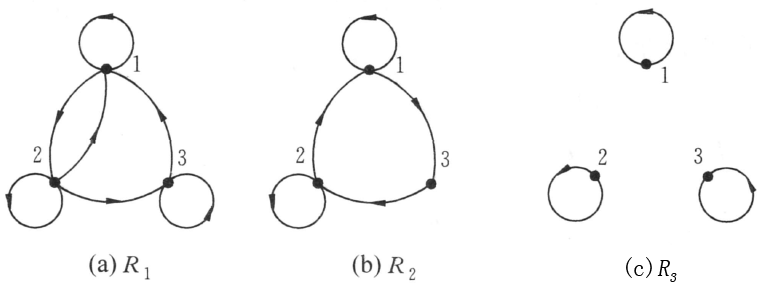
\includegraphics[width=5cm,height=4cm,keepaspectratio]{figures/image28.png}\par}\medskip

A B C:①自反的，对称的，传递的 ②反自反的，对称的 ③自反的

\begin{enumerate}
\setcounter{enumi}{3}
\item
  反对称的 ⑤对称的 ⑥自反的，对称的，反对称的，传递的
\end{enumerate}

4. 设 S=\{Ф，\{1\}，\{1，2\}\}，则有

（1）（A）\(\in\)S （2） (B) \(\subseteq\)S

（3） P(S)有（C）个元数。 （4）（D）既是 S 的元素，又是 S 的子集

A: ① \{1,2\} ② 1 B: ③\{\{1,2\}\} ④\{1\}

C: ⑤ 3 ⑥ 6 ⑦ 7 ⑧ 8 D: ⑨ \{1\} ⑩Ф

\pdfbookmark[1]{二、证明（本大题共2小题，第1小题10分，第2小题10分，总计20分）}{section58}

\par\medskip{\heiti

二、证明（本大题共 2 小题，第 1 小题 10 分，第 2 小题 10 分，总计 20 分）

\par}\smallskip

1、用等值演算算法证明等值式 (p\(\land\)q)\(\lor\)(p\(\land\)\(\neg\)q)\(\Leftrightarrow\)p

2、构造下面命题推理的证明

如果今天是星期三，那么我有一次英语或数学测验；如果数学老师有事，那么没有数学测验；今天是星期三且数学老师有事，所以我有一次英语测验。

\pdfbookmark[1]{三、计算（本大题共4小题，第1小题5分，第2小题10分，第3小题15分，}{section62}

\par\medskip{\heiti

三、计算（本大题共 4 小题，第 1 小题 5 分，第 2 小题 10 分，第 3 小题 15 分，

\par}\smallskip

总计 30 分）

1、设\(P\left( {x,y} \right)\text{为}x\text{整除}y\text{，}\allowbreak Q(x)\text{为}x < 2\text{，个体域为}\left\{ {1\text{，}\allowbreak 2} \right\}\)，求公式：

\(\left( {\forall x} \right)\left( {\exists y} \right)\left( P\left( {x,y} \right)\rightarrow Q(x) \right)\)的真值。

2、设集合\(A = \left\{ {1,2,3,4} \right\},A\)上的关系 \(R = \left\{ {\left\langle {1,1} \right\rangle,\left\langle {1,2} \right\rangle,\left\langle {2,1} \right\rangle,\left\langle {2,3} \right\rangle,\left\langle {3,4} \right\rangle} \right\}\)，求出它的自反闭包，对称闭包和传递闭包。

3、设\(A = \left\{ {1,2,4,8,12,24,} \right\}\)上的整除关系\(R = \left\{ {\left\langle {a_{1},a_{2}} \right\rangle\left| {a_{1},a_{2} \in A,a_{1}\text{整除}a_{2}} \right.} \right\}\)，\(R\)是否为\(A\)上的偏序关系？若是，则：

1、画出\(R\)的哈斯图；（10 分）

2、求它的极小元，最大元，极大元，最大元。（5 分）

\pdfbookmark[1]{四、用推导法求公式left( left( prightarrow q right)rightarrow p right)}{section70}

四、用推导法求公式\(\left( \left( p\rightarrow q \right)\rightarrow p \right)\)的主析取范式和主合取范式。（本大题 10 分）

\end{document}
